\fancyhead[L]{\textbf{32}\qquad\textbf{CHƯƠNG 1}\quad HÀM SỐ VÀ MÔ HÌNH}
\fancyhead[R]{}

\noindent
\begin{center}
    {\large\textbf{\textsf{Bảng 3}}\quad \textbf{\textsf{Các họ hàm số cơ bản và đồ thị của chúng}}}
\end{center}

\vspace{-6pt}
\noindent
\begin{center}
\renewcommand{\arraystretch}{1.0}
\setlength{\tabcolsep}{3pt}
\begin{tabular}{|>{\centering\arraybackslash}m{0.18\textwidth}|>{\centering\arraybackslash}m{0.78\textwidth}|}
\hline
\cellcolor[RGB]{235,243,250}
\textbf{\textsf{\color{stewartcyan}Hàm tuyến tính}}\\[3pt]
$f(x) = mx + b$
&
\vspace{2pt}
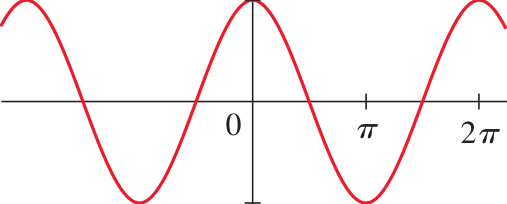
\includegraphics[height=65pt,keepaspectratio]{images/p0067_graph_7.png}\qquad
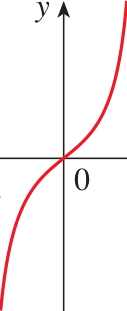
\includegraphics[height=65pt,keepaspectratio]{images/p0067_graph_8.png}
\vspace{2pt}
\\ \hline
\cellcolor[RGB]{235,243,250}
\textbf{\textsf{\color{stewartcyan}Hàm lũy thừa}}\\[3pt]
$f(x) = x^n$
&
\vspace{2pt}
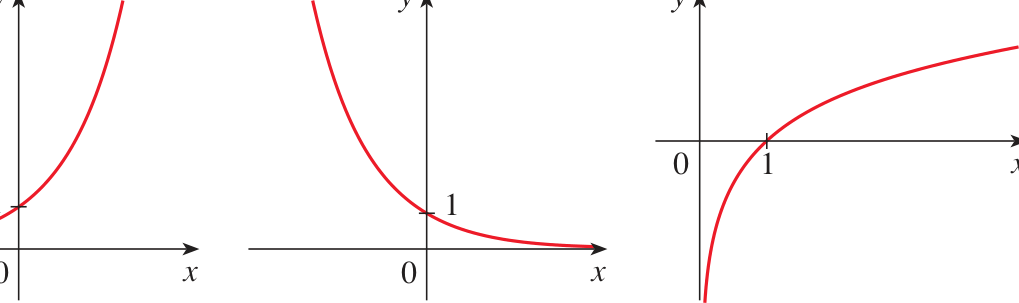
\includegraphics[height=65pt,keepaspectratio]{images/p0067_graph_1.png}
\vspace{2pt}
\\ \hline
\cellcolor[RGB]{235,243,250}
\textbf{\textsf{\color{stewartcyan}Hàm căn thức}}\\[3pt]
$f(x) = \sqrt[n]{x}$
&
\vspace{2pt}
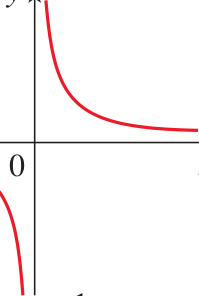
\includegraphics[height=65pt,keepaspectratio]{images/p0067_graph_10.png}\qquad
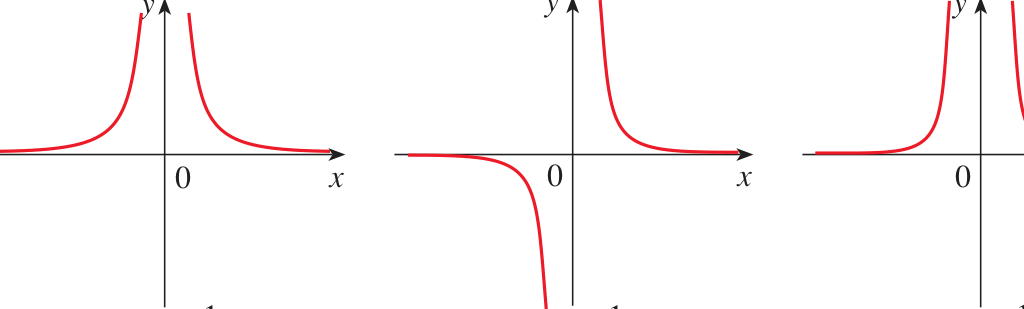
\includegraphics[height=65pt,keepaspectratio]{images/p0067_graph_11.png}
\vspace{2pt}
\\ \hline
\cellcolor[RGB]{235,243,250}
\textbf{\textsf{\color{stewartcyan}Hàm nghịch đảo}}\\[3pt]
$f(x) = \dfrac{1}{x^n}$
&
\vspace{2pt}
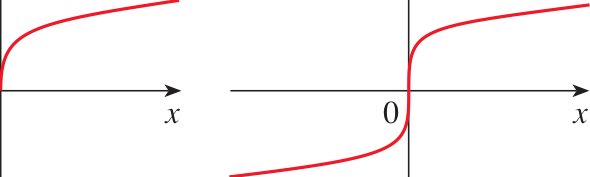
\includegraphics[height=65pt,keepaspectratio]{images/p0067_graph_9.png}
\vspace{2pt}
\\ \hline
\cellcolor[RGB]{235,243,250}
\textbf{\textsf{\color{stewartcyan}Hàm mũ và}}\\[1pt]
\textbf{\textsf{\color{stewartcyan}hàm logarit}}\\[3pt]
$f(x) = b^x$\\[2pt]
$f(x) = \log_b x$
&
\vspace{2pt}
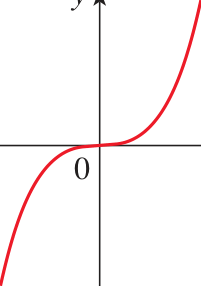
\includegraphics[height=65pt,keepaspectratio]{images/p0067_graph_5.png}\enspace
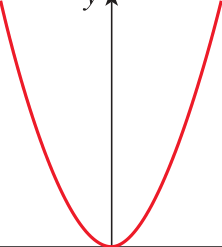
\includegraphics[height=65pt,keepaspectratio]{images/p0067_graph_3.png}\enspace
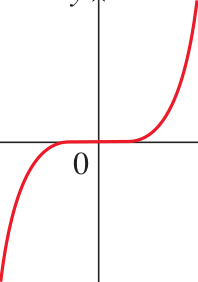
\includegraphics[height=65pt,keepaspectratio]{images/p0067_graph_6.png}\enspace
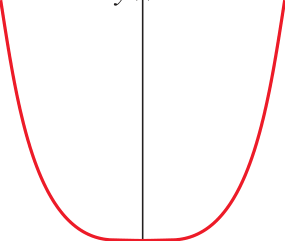
\includegraphics[height=65pt,keepaspectratio]{images/p0067_graph_4.png}
\vspace{2pt}
\\ \hline
\cellcolor[RGB]{235,243,250}
\textbf{\textsf{\color{stewartcyan}Hàm lượng giác}}\\[3pt]
$f(x) = \sin x$\\[2pt]
$f(x) = \cos x$\\[2pt]
$f(x) = \tan x$
&
\vspace{2pt}
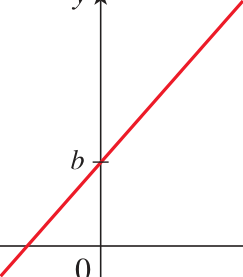
\includegraphics[height=65pt,keepaspectratio]{images/p0067_graph_2.png}
\vspace{2pt}
\\ \hline
\end{tabular}
\end{center}